\begin{figure}
  \center
 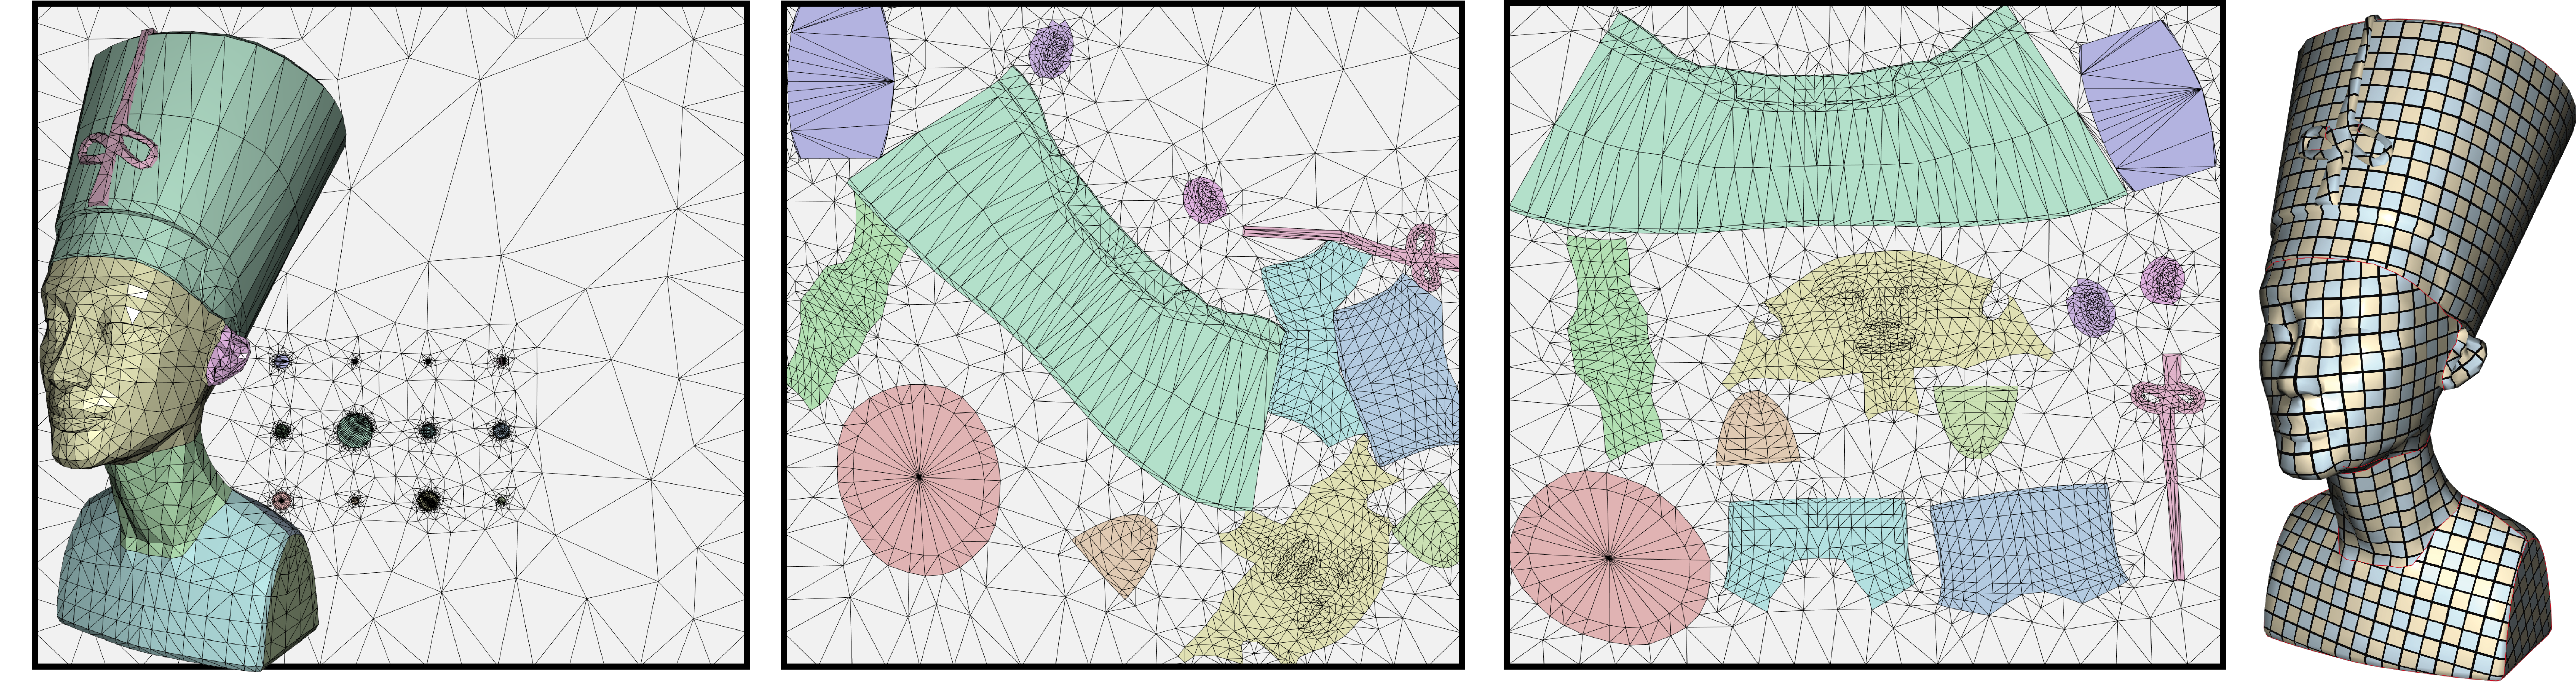
\includegraphics[width=\textwidth]{scaf-tex/figs/teaser}
 \caption{The Nefertiti model with prescribed seams is UV mapped by our algorithm. Each chart is bijective mapped into a circle or ring with Tutte's embedding and achieves minimal distortion in less than a second. The layout is further improved interactively and the final parametrized model is shown on the right. Our approach guarantees a valid UV map with no inverted elements or overlapping triangles. See the attaching video for the optimization and manual interaction.
}
 \label{scaf:fig:teaser}
\end{figure}

\section{Introduction}

The computation of discrete maps is a fundamental problem in computer graphics that has been extensively studied in the last three decades. The problem is challenging due to the large solution space
and the non-linearity of the desired properties (\revision{in both} distortion measures and constraints). Algorithms for robustly and efficiently computing locally injective (i.e. non-flipping) maps have been only recently introduced \cite{Lipman:2012,Kovalsky:2016,rabinovich2017scalable} and are now having a major impact in many research areas outside of traditional texture mapping, including remeshing \cite{Bommes:2013}, image editing \cite{Poranne:2014}, and cultural heritage \cite{Pal:2014}.

In this chapter, we consider the problem of generating bijective maps, i.e. locally injective maps with \revision{non-intersecting boundaries} %no self-overlapping triangles. 
This is a difficult problem, exacerbated by the fact that any pair of \revision{boundary elements could overlap, leading to non-linear constraints whose number is quadratic in the size of the boundary}. %triangles could potentially overlap, leading to a quadratic number of non-linear constraints to satisfy \revision{(yet, with locally injectivity, number of constraints can be seen as linear in terms of boundary elements \cite{Lipman:2013ArXiv}).} 
This problem is usually tackled by iteratively deforming an existing map, checking for overlaps after each step, and then preventing the overlap using constraints \cite{Harmon:2011} or penalty forces \cite{harmon2010robust}. These methods require a spatial acceleration structure to find the candidate pairs of overlapping elements and a resolution strategy that updates the map while avoiding the detected overlaps. \revision{However, t}he newly computed displacement might \revision{in turn} lead to new overlaps, and this process \revision{has to be} performed iteratively \revision{in the hope that} no  collisions are \revision{left}. Difficult cases with many collisions might requires tens or hundreds of iterations before all the candidate intersecting pairs are detected.

Our approach sidesteps the need to find candidate self-intersections \revision{based on a} simple observation: if the the entire ambient space \revision{(with a fixed simple boundary)} is tessellated, then local injectivity implies global bijectivity \cite{Zhang:2005,Lipman:2013ArXiv,Muller:2015}. We \revision{thus} propose an optimization framework based on this idea \revision{making it possible to} leverage recent techniques for \revision{locally} injective maps; our algorithm is simple to implement, robust, and two orders of magnitude faster than competing methods.

\paragraph{Overview.} Given an input bijective map represented by a discrete triangle mesh and its mapped vertex locations, we create a new scaffold mesh for a bounding box that contains the initial, mapped triangle mesh (Figure \ref{scaf:fig:teaser}) and conforms to its boundary. We then optimize for the desired property of the map (such as distortion, positional constraints, etc.) while ensuring that no triangle will flip. This property is achieved using a variational formulation that combines a user-defined energy for the map with a regularization term that allows the scaffold to freely deform without hindering the optimization of the map properties. During the optimization, we refine and optimize the connectivity of the scaffold mesh to prevent possible locking situations.

\revision{While a scaffold mesh has been already used in previous works \cite{Zhang:2005,Misztal:2012,Muller:2015}, we propose to use an isometric distortion energy on the scaffold mesh, with the reference reset to the current rest pose at each iteration, and an online remeshing strategy. Our scaffold energy aims for "isometry to the current iteration", which resembles how plasticity is usually modeled in elasto-plastic simulations --- this leads to a global and natural deformation of the scaffold elements that opens up space for the evolving boundary and allows for an efficient optimization using recent numerical methods for locally injective maps \cite{rabinovich2017scalable}.}

We demonstrate the practical utility of our algorithm in the context of single patch mesh parametrization by producing distortion minimizing bijective maps for a collection of \revision{119} challenging models. Our algorithm is ideal to compute tight UV maps for models with multiple connected components and seams as we demonstrate in our interactive texture packing experiments. Our algorithm can also be easily extended to 3D by replacing the triangular scaffold with one composed of tetrahedra. For the 3D case, we show that our method can be used to deform surfaces preventing self-intersections and to remove self-intersection from existing genus-0 surfaces when paired with a mean conformalized flow \cite{Kazhdan:2012,Sacht:2013}.

In the additional material, we provide a video (showing the optimization iterations) and the input/output meshes for each figure in the paper. To foster replicability of results, we will release an open-source reference implementation of our algorithm. 


\paragraph{Contribution.}
\begin{itemize}
\vspace{-1em}
\item We enhance the idea of scaffolding to the context of efficient geometric optimization with the "isometry to the current iteration" energy. This allows scaffold elements to freely open up space for the chart boundary to take larger steps than otherwise possible (Figure 12), as well as oblivious to the triangulation at each iteration.
\item To the best of our knowledge, ours is the first method that can bijectively parameterize large, complex models efficiently and robustly.
\item Our method provides an intuitive and simple way to prevent degenerate elements, which is required to avoid locking (different from \cite{Muller:2015}, where they must allow flip to exert force), and handles challenging cases such as those in Figure 5. 
Our formulation unifies geometric optimization problems in 2D/3D
%\item 
%Our work is also greatly motivated by practical considerations: we are not aware of any method that can robustly/efficiently compute bijective maps in 2D and 3D, which is fundamental and appears in many graphics and geometry processing tasks. We believe our proposal is a major step forward in solving this problem, simple to implement, and extremely robust.
\end{itemize}
